\section{Halo-independent bounds}\label{sec:21.2}

A dark-matter particle of \SI{2}{MeV} can make an electron--hole pair in silicon only if it moves faster than \SI{325}{km.s^{-1}} in the laboratory, and a second pair only above \SI{466}{km.s^{-1}}, against the largest speed of the standard halo, $v_{\mathrm{max}} = \SI{794.5}{km.s^{-1}}$. A limit at that mass is therefore a statement about the fast part of the dark matter in the solar neighborhood, the part of the halo that \cref{sec:1.2} found least certain: changing the escape speed by \SI{25}{km.s^{-1}} changes $\eta$ at \SI{760}{km.s^{-1}} by a factor of 2.26 or 0.10. A statement that holds for every velocity distribution avoids the question. Because every count is a linear functional of $f_\chi$ (\cref{eq:21.1-functional}), the distributions that a null result allows form a convex set, and the largest value of any other linear quantity over that set is a semi-infinite linear program, with finitely many constraints on a measure over a continuum, the problem of \cref{app:C.12}. For silicon at 2 and \SI{10}{MeV}, dropping the halo model costs a factor of 2.0 to 3.7 in the bulk of the halo and orders of magnitude near $v_{\mathrm{max}}$.

\subsection{Stream kernels and the linear program}\label{sec:21.2-program}

The exposure-averaged rate \cref{eq:21.1-exposure} is an integral over galactic velocities $\vect{w}$ of the distribution $f_{\mathrm{gal}}$ times a kernel. Multiplied by the exposure $M_{\mathrm{det}}t_{\mathrm{exp}}$ it is a count. The local density, the cross-section and the mass multiply every rate in the combination $\rho_\chi\sigmae/\mchi$, which no count can separate from the normalization of $f_{\mathrm{gal}}$; the mass enters the kinematics as well, and the analysis is done at fixed $\mchi$. We therefore absorb the combination into a nonnegative measure $\Xi$ on the ball $\mathcal{B} = \{|\vect{w}| \le v_{\mathrm{esc}}\}$ and divide the kernel by $\sigmae$ (\cref{app:D.46}):
\begin{equation}
  \dd\Xi(\vect{w}) = \frac{\rho_\chi\sigmae}{\mchi}\,f_{\mathrm{gal}}(\vect{w})\,\dd^3w , \qquad
  \mathsf{k}_i(\vect{w}) = \frac{M_{\mathrm{det}}t_{\mathrm{exp}}}{\rho_T\,\sigmae}\,\bigl\langle\varGamma_i\bigl(\vect{w} - \vect{v}_{\mathrm{E}}(t)\bigr)\bigr\rangle_t ,
  \label{eq:21.2-stream}
\end{equation}
with $\varGamma_i$ the rate kernel \cref{eq:21.1-kernel} for bin $i$ of the observable. The expected count in bin $i$ is then $\int\mathsf{k}_i\,\dd\Xi$. The \emph{stream kernel} $\mathsf{k}_i(\vect{w})$ is the count that a single stream of unit $\Xi$-mass at $\vect{w}$ would leave in bin $i$; it contains the coupling up to its strength, the response, the final-state weights and the exposure, and nothing about the halo. A measured null result in bin $i$ becomes the constraint $\int\mathsf{k}_i\,\dd\Xi \le N_i^{\mathrm{up}}$, with $N_i^{\mathrm{up}}$ the upper count of \cref{sec:1.5} at the chosen confidence.

The quantity to bound is a second linear functional, $\int\mathsf{f}\,\dd\Xi$: the mean inverse speed above $u_0$ in the laboratory, the count of a second experiment, or a modulation amplitude. The mean inverse speed is the object of the standard halo-independent analysis,
\begin{equation}
  \tilde\eta(u_0) = \int\frac{\Theta(|\vect{w} - \vect{v}_{\mathrm{E}}| - u_0)}{|\vect{w} - \vect{v}_{\mathrm{E}}|}\,\dd\Xi(\vect{w}) = \frac{\rho_\chi\sigmae}{\mchi}\,\eta(u_0) ,
  \label{eq:21.2-etatilde}
\end{equation}
which is $\tilde\eta$ of \cref{app:A.8} with $\vect{v}_{\mathrm{E}}$ held fixed. Its value for the standard halo at a given $\sigmae$ is a curve in the plane of $u_0$ and $\tilde\eta$, and a bound on $\tilde\eta$ at every $u_0$ is the halo-independent counterpart of an exclusion curve. The count expected in a second experiment, $\mathsf{f} = \mathsf{k}^{\mathrm{B}}_j$, compares two targets, or one crystal at two orientations, without a halo model. A modulation amplitude, the difference of the kernels of two time bins, is a signed functional, bounded only if every stream on which it is positive is seen by some bin. The program is \cref{eq:C.12-sip} with these kernels.

By \cref{app:C.12}, any vector $\boldsymbol\lambda \ge 0$ with $\sum_i\lambda_i\mathsf{k}_i \ge \mathsf{f}$ on all of $\mathcal{B}$, a \emph{dual certificate}, proves $\int\mathsf{f}\,\dd\Xi \le \int\sum_i\lambda_i\mathsf{k}_i\,\dd\Xi \le \sum_i\lambda_iN_i^{\mathrm{up}}$ for every allowed halo at once, \cref{eq:C.12-certificate}. Checking it needs one function evaluated on the ball, not the optimizer that produced it. And the optimum is attained by a halo of at most $n$ streams for $n$ bins, $\Xi^* = \sum_a\xi_a\delta_{\vect{w}_a}$ with $\Xi$-masses $\xi_a$, placed at the zeros of the dual function $\mathsf{g}_\lambda = \sum_i\lambda_i\mathsf{k}_i - \mathsf{f}$. The extremal halos are therefore cold streams, far from any equilibrium model, and the bound holds for every halo because it holds for them. With the normalization of $f_\chi$ as an extra equality constraint the optimum allows one more stream~\cite[Eqs.~(14)--(19)]{ibarra2017optimized}, and any likelihood, not only a bound, is maximized by a sum of streams~\cite{gelmini2017unified}.

All bins of a search constrain one halo, so a bound derived from them is a statement about the event that every bin stays below its $N_i^{\mathrm{up}}$. If each bin is set at confidence $1 - \alpha_i$, that event has probability at least $1 - \sum_i\alpha_i$ by the union bound, and the bounds at all $u_0$ hold together at that level. The examples below use three pair bins with $N_i^{\mathrm{up}} = \ln 30 = 3.401$ each, the zero-event Poisson limit at 96.7 percent, so that the three bins hold jointly at 90 percent or more.

\subsection{The bound for a speed-only response}\label{sec:21.2-iso}

For a response averaged over the directions of $\vect{q}$, as in the crystal form factor of \cref{sec:10.1}, and with $\vect{v}_{\mathrm{E}}$ fixed, the stream kernel depends only on the laboratory speed $v = |\vect{w} - \vect{v}_{\mathrm{E}}|$. By \cref{eq:21.1-gammav} it is $\mathsf{k}_i(v) = \mathcal{A}_i(v)/v$, with the \emph{step column}
\begin{equation}
  \mathcal{A}_i(v) = \frac{M_{\mathrm{det}}t_{\mathrm{exp}}}{\rho_T\,\sigmae}\,v\,\varGamma_i(v) = \frac{M_{\mathrm{det}}t_{\mathrm{exp}}}{\rho_T\,\sigmae}\int\dd\omega\int\frac{q\,\dd q}{4\pi^2}\,\bar s_i(q,\omega)\,\Theta\bigl(v - \vmin(q,\omega)\bigr) ,
  \label{eq:21.2-column}
\end{equation}
where $\bar s_i$ is the angle-averaged response contracted with $\mathfrak{D}$ and weighted with the probability $P(i|\Lambda)$ of landing in bin $i$. The column is the count in bin $i$ for the step $\tilde\eta(u) = \Theta(v - u)$: all of $\tilde\eta$ sits below the speed $v$, the halo of a single stream at $v$. In silicon with the loss function of \cref{sec:10.2}, written as a crystal form factor by \cref{eq:A.8-fcrys,eq:4.4-SL}, the prefactor $M_{\mathrm{det}}t_{\mathrm{exp}}\,\alpha m_e^2/(M_{\mathrm{cell}}\mu_{\chi e}^2)$, with $M_{\mathrm{cell}}$ the mass of the two-atom unit cell, turns the column into a sum over the table, and $\mathcal{A}_i$ comes out in years for $\tilde\eta$ in inverse years. For a positive response the column never decreases with $v$ (\cref{eq:D.46-monotone}), since a faster particle reaches every pair that a slower one does (\cref{sec:21.1-eta}).

Monotonicity solves the program:
\begin{keyresult}[Halo-independent bound for a speed-only response]
For a response that depends only on $|\vect{q}|$, nonnegative bin weights, a fixed $\vect{v}_{\mathrm{E}}$, $0 < u_0 \le v_{\mathrm{max}}$ and $\max_i\mathcal{A}_i(u_0) > 0$, every velocity distribution allowed by the bins satisfies
\begin{equation}
  \tilde\eta(u_0) \le \min_i\frac{N_i^{\mathrm{up}}}{\mathcal{A}_i(u_0)} ,
  \label{eq:21.2-hib}
\end{equation}
and the bound is attained. The optimal halo is one stream at laboratory speed $u_0$ in any allowed direction, and the certificate is $\lambda_j = 1/\mathcal{A}_j(u_0)$ on the minimizing bin $j$, zero on the others.
\end{keyresult}
\noindent \Cref{app:D.46} gives the proof: the stream is feasible and reaches the bound, and the certificate holds because $\mathcal{A}_j(v) \ge \mathcal{A}_j(u_0)$ for $v \ge u_0$. With several bins the minimum over bins is the exact optimum, not an estimate, because one dual weight certifies it; the other bins are not saturated by the optimal stream and carry no weight. A column that decreases somewhere, which a truncated response with negative pieces can produce, leaves the single-bin value $N_i^{\mathrm{up}}/\inf_{v \ge u_0}\mathcal{A}_i(v)$ of \cref{eq:C.12-onebin} and voids the closed form for several bins (\cref{app:D.46}). And a bound on the galactic speed integral $\int\Theta(|\vect{w}| - u_0)|\vect{w}|^{-1}\dd\Xi$, in place of the laboratory speed $|\vect{w} - \vect{v}_{\mathrm{E}}|$ on which the kernel depends, is a different program, and \cref{eq:21.2-hib} does not answer it.

\Cref{fig:21-hib} applies \cref{eq:21.2-hib} to a silicon search of one kilogram-year that records no event in the one-, two- and three-pair bins, for a heavy mediator. A deposit $\omega$ lands in bin $i$ with the probability $P_{\mathrm{casc}}(i|\omega)$ of the cascade of \cref{sec:18.3}, the book's calibrated model with $\Eg = \SI{1.160}{eV}$ and \SI{3.749}{eV} per pair, computed for the seed of a dark-matter kick and applied at every $q$. The probability of the one-pair bin exceeds one half from 1.2 to \SI{6.2}{eV}, that of the two-pair bin from 6.3 to \SI{9.5}{eV} and that of the three-pair bin from 9.7 to \SI{13.1}{eV}, and a second pair is possible from about \SI{2.5}{eV}. Each bin gives a curve $N_i^{\mathrm{up}}/\mathcal{A}_i(u_0)$ that comes down from infinity at the onset speed of the bin, the smallest $\vmin$ among the pairs it can contain, and flattens as the column saturates; the bound is their lower envelope. At \SI{10}{MeV} the one-pair bin sets it below \SI{481.8}{km.s^{-1}}, the two-pair bin up to \SI{757.3}{km.s^{-1}} and the three-pair bin above. At \SI{2}{MeV} the one-pair bin sets it at every speed: the two-pair bin opens at \SI{465.9}{km.s^{-1}} and the three-pair bin at \SI{611.8}{km.s^{-1}}, and at $v_{\mathrm{max}}$ their columns are 2.4 and 206 times smaller. The dashed curves are $\tilde\eta$ of the standard halo at the cross-section where it first reaches $N_i^{\mathrm{up}}$ in some bin: $\sigmae = \SI{1.17e-41}{cm^2}$ at \SI{10}{MeV} and \SI{1.12e-40}{cm^2} at \SI{2}{MeV}, both set by the one-pair bin.

The standard curve lies below the bound at every $u_0$, as it must. The count of any halo in bin $j$ is $\int_0^\infty\tilde\eta(u)\,\dd\mathcal{A}_j(u)$, \cref{eq:21.1-etaform} in these variables, and since $\tilde\eta$ never increases and $\mathcal{A}_j$ never decreases, it is at least $\tilde\eta(u_0)\mathcal{A}_j(u_0)$. A halo that crossed the bound at some $u_0$ would overshoot $N_j^{\mathrm{up}}$. The ratio of the bound to the standard curve is the cost of dropping the halo model. It is smallest at \SI{381}{km.s^{-1}} for \SI{10}{MeV}, a factor 2.00, and near \SI{635}{km.s^{-1}} for \SI{2}{MeV}, a factor 3.70. Toward $v_{\mathrm{max}}$ it opens to 9.6 at \SI{600}{km.s^{-1}} and 63 at \SI{700}{km.s^{-1}} for \SI{10}{MeV}, because the standard halo has few particles there while a stream can put all its density at one speed. The curves hold for an exposure at the reference Earth speed; over a year the standard curve near $v_{\mathrm{max}}$ follows the year average of \cref{sec:21.1}, 1.06 times higher at \SI{700}{km.s^{-1}}.

\begin{figure}[tbp]
  \centering
  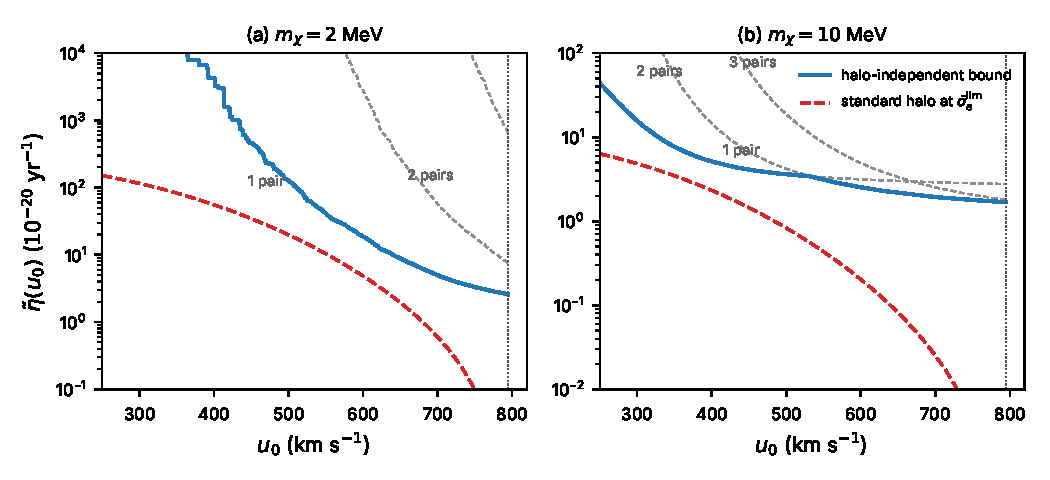
\includegraphics[width=\linewidth]{figures/ch21/fig21_2.pdf}
  \caption{Halo-independent bound on $\tilde\eta(u_0) = \rho_\chi\sigmae\eta(u_0)/\mchi$ for silicon, \cref{eq:21.2-hib} (solid), against $\tilde\eta$ of the standard halo at the cross-section of its own limit (dashed), for (a) $\mchi = \SI{2}{MeV}$ and (b) \SI{10}{MeV}, heavy mediator. Search: one kilogram-year at the reference Earth speed, no events in the one-, two- and three-pair bins, with the bin probabilities of the energy-only cascade of \cref{sec:18.3} (\SI{3.749}{eV} per pair), $N_i^{\mathrm{up}} = \ln 30$ in each bin, jointly at least 90 percent confidence. Gray dashed: single-bin bounds $N_i^{\mathrm{up}}/\mathcal{A}_i(u_0)$, labeled by the number of pairs; the solid curve is their lower envelope. Step columns from the direction-averaged random-phase loss function with local fields of Knapen, Kozaczuk and Lin (\cref{sec:10.2}), from \SI{1.17}{eV}. Standard halo: $v_0 = 238$, $v_{\mathrm{esc}} = \SI{544}{km.s^{-1}}$, $v_{\mathrm{E}}^{\mathrm{ref}} = \SI{250.5}{km.s^{-1}}$, at $\sigmae = \SI{1.12e-40}{cm^2}$ (a) and \SI{1.17e-41}{cm^2} (b). Dotted: $v_{\mathrm{max}} = \SI{794.5}{km.s^{-1}}$.}
  \label{fig:21-hib}
\end{figure}

\begin{workedexample}{One stream saturating a bound}\label{we:21-stream}
Take silicon at $\mchi = \SI{10}{MeV}$, a heavy mediator, the search of \cref{fig:21-hib} and $u_0 = \SI{500}{km.s^{-1}}$. The reduced mass is $\mu_{\chi e} = \SI{486.2}{keV}$, and the prefactor of the column, $M_{\mathrm{det}}t_{\mathrm{exp}}\,\alpha m_e^2/(M_{\mathrm{cell}}\mu_{\chi e}^2)$, is \SI{8.64e22}{yr} for one kilogram-year. Summing the cells of the table with $\vmin \le \SI{500}{km.s^{-1}}$, each weighted with its bin probability, gives
\begin{equation*}
  \mathcal{A}_1 = \SI{3.10e19}{yr} , \qquad \mathcal{A}_2 = \SI{3.48e19}{yr} , \qquad \mathcal{A}_3 = \SI{8.88e18}{yr} ,
\end{equation*}
for the one-, two- and three-pair bins. Divided into $N^{\mathrm{up}} = 3.401$ they give \num{1.10e-19}, \num{9.78e-20} and \SI{3.83e-19}{yr^{-1}}. The two-pair bin is tightest, and
\begin{equation*}
  \tilde\eta(\SI{500}{km.s^{-1}}) \le \frac{3.401}{\SI{3.48e19}{yr}} = \SI{9.78e-20}{yr^{-1}} .
\end{equation*}
The halo that reaches it is one stream at a laboratory speed of \SI{500}{km.s^{-1}}, $1.668\times10^{-3}$ in natural units, with $\Xi$-mass $\xi_1 = u_0N^{\mathrm{up}}/\mathcal{A}_2 = \SI{1.63e-22}{yr^{-1}}$. It leaves 3.03 events in the one-pair bin, 3.40 in the two-pair bin and 0.87 in the three-pair bin: only the two-pair bound is saturated. Its galactic speed lies between \num{249.5} and \SI{750.5}{km.s^{-1}} depending on its direction, and the directions against the Earth's motion are inside the escape speed.

The certificate is $\lambda_2 = 1/\mathcal{A}_2 = \SI{2.88e-20}{yr^{-1}}$ per event, $\lambda_1 = \lambda_3 = 0$, with value $\lambda_2N^{\mathrm{up}} = \SI{9.78e-20}{yr^{-1}}$, equal to the stream's. It is valid because $\mathcal{A}_2(v)/\mathcal{A}_2(u_0)$ never drops below 1 between \num{500} and \SI{794.5}{km.s^{-1}}, where it rises to 2.15.

The standard halo at its own limit, $\sigmae = \SI{1.17e-41}{cm^2}$, set by the one-pair bin, has $\tilde\eta(\SI{500}{km.s^{-1}}) = \SI{2.60e-20}{yr^{-1}}$, a factor 3.76 below the bound. The factor has two parts, read in the two-pair bin that sets the bound. The standard halo leaves only 2.47 events there, because the one-pair bin stops it first, and only 1.27 of them come from particles faster than \SI{500}{km.s^{-1}}; the bin allows $N^{\mathrm{up}} = 3.401$, a factor $3.401/1.266 = 2.69$ above what those particles use. And the fast particles move above \SI{500}{km.s^{-1}}, where the column is larger, so they produce 1.40 times the count of a stream at exactly \SI{500}{km.s^{-1}} with the same $\tilde\eta$. The stream avoids both losses, and $2.69 \times 1.40 = 3.76$.
\end{workedexample}

\subsection{Directional responses in the laboratory}\label{sec:21.2-dir}

A crystal resolves directions. Its response depends on $\hat{\vect{q}}$ in crystal axes, the crystal turns with the Earth, and a stream fixed in the galactic frame sweeps a cone of crystal directions every sidereal day (\cref{sec:11.7}). The stream kernel then depends on the direction of the stream, there is no step column, and the program has to be solved. Take a cubic crystal and a coupling that depends on $|\vect{q}|$ alone. The bin-weighted response is then $\bar s_i[1 + \sum_\ell a^i_\ell Y^{\mathrm{c}}_\ell(\hat{\vect{q}})]$, with the cubic harmonics of \cref{app:C.3}, $\ell = 4, 6, 8, \dots$ The energy delta function confines $\hat{\vect{q}}$ to a circle about the stream direction, at the angle $\arccos(\vmin/v)$, and the average of a harmonic over that circle is $P_\ell(\vmin/v)Y^{\mathrm{c}}_\ell(\hat{\vect{v}})$, \cref{eq:D.46-circle}. The kernel of a stream of velocity $\vect{v}$ in crystal axes is
\begin{equation}
  \mathsf{k}_i(\vect{v}) = \frac{M_{\mathrm{det}}t_{\mathrm{exp}}}{\rho_T\,\sigmae\,v}\int\dd\omega\int\frac{q\,\dd q}{4\pi^2}\,\bar s_i(q,\omega)\Bigl[1 + \sum_{\ell \ge 4}a^i_\ell(q,\omega)\,P_\ell\Bigl(\frac{\vmin}{v}\Bigr)Y^{\mathrm{c}}_\ell(\hat{\vect{v}})\Bigr]\Theta\bigl(v - \vmin(q,\omega)\bigr) ,
  \label{eq:21.2-multipole}
\end{equation}
before the average over the exposure (\cref{app:D.46}). Pairs with $\vmin$ close to $v$ are reached only by momentum transfers along the stream, $P_\ell \to 1$, and carry the full anisotropy of the response. Pairs with $\vmin \ll v$ are reached on a wide circle, and their anisotropy is reduced by $P_\ell(\vmin/v)$, which for $\ell \ge 4$ is at most 0.375 in magnitude as $\vmin/v \to 0$. The anisotropy of the kernel is therefore largest near the onset speed of each bin, where every reachable pair has $\vmin \approx v$.

The exposure average turns $Y^{\mathrm{c}}_\ell(\hat{\vect{v}})$ into its mean over the crystal directions that the stream visits. With $\vect{v}_{\mathrm{E}}$ fixed, a stream of laboratory speed $v$ and declination $\delta_{\mathrm{dec}}$ visits, over one sidereal day, the directions of \cref{eq:1.2-local} at all hour angles, and the mean depends on $\delta_{\mathrm{dec}}$, the latitude and the orientation of the crystal only. Streams with all right ascensions at a given $\delta_{\mathrm{dec}}$ therefore have the same kernel, and the program may place a stream at whichever right ascension the galactic support allows. That support, $|\vect{v} + \vect{v}_{\mathrm{E}}| \le v_{\mathrm{esc}}$, allows the declination $\delta_{\mathrm{dec}}$ at speed $v$ for some right ascension if $v^2 + |\vect{v}_{\mathrm{E}}|^2 - 2v|\vect{v}_{\mathrm{E}}|\cos(\delta_{\mathrm{dec}} + \delta_{\mathrm{E}}) \le v_{\mathrm{esc}}^2$, with $\delta_{\mathrm{E}} = 47.5^\circ$ the declination of $\vect{v}_\odot$ (\cref{sec:1.2}); the cosine is that of the smallest angle between $-\vect{v}$ and $\vect{v}_{\mathrm{E}}$ over right ascension. At $v_{\mathrm{max}}$ only $\delta_{\mathrm{dec}} = -\delta_{\mathrm{E}}$ remains, a stream that moves opposite to the Earth and arrives from the direction toward which the Sun moves. The program reduces to two variables, the speed and the declination of the stream.

\Cref{lim:21.2a} solves it for silicon at \SI{2}{MeV}, where every momentum transfer lies in the range of the model response of \cref{sec:11.7}. The isotropic part of the kernel comes from the loss function of \cref{fig:21-hib}. The ratios $a_\ell$ for $\ell = 4, 6, 8$ come from the cubic-harmonic components of the independent-particle structure factor of the empirical-pseudopotential model of \cref{sec:11.7}, applied at the same $(q,\omega)$. They are a model, with a gap of \SI{0.82}{eV} and no local fields, so the plot tests the method rather than measures silicon. The detector sits at \ang{45} north with $[001]$ vertical, $[100]$ east and $[010]$ north, the orientation of \cref{we:11-daily}, and records the search of \cref{fig:21-hib} in its one- and two-pair bins, integrated over sidereal time; the three-pair bin, open only above \SI{612}{km.s^{-1}} at this mass, never binds.

\begin{limitbox}[Speed-only bound against a directional response][lim:21.2a]
For a response averaged over the directions of $\vect{q}$ and a laboratory-frame stream~\cite[Eqs.~(A1)--(A2)]{fox2011integrating}: $\tilde\eta(u_0) \le \min_iN_i^{\mathrm{up}}/\mathcal{A}_i(u_0)$, \cref{eq:21.2-hib}. The formula ignores the anisotropy of the crystal; the plot shows how far the bound of the directional program departs from it.
\par\smallskip
{\centering
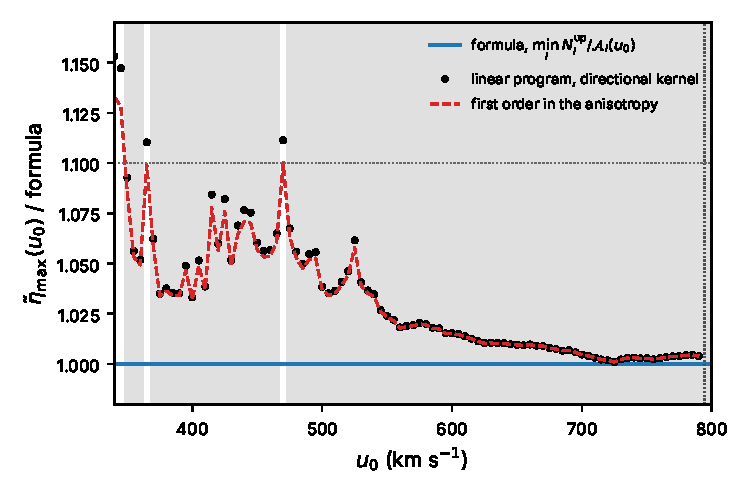
\includegraphics[width=\linewidth]{figures/ch21/limit21_2a.pdf}
\captionof{figure}{Largest $\tilde\eta(u_0)$ allowed by a silicon search over all halos, divided by the formula of the box (solid line at 1), against $u_0$. Dots: the fuller result, the linear program over galactic-frame streams with the direction-dependent kernel \cref{eq:21.2-multipole} of a crystal at \ang{45} north ($[001]$ up, $[100]$ east), integrated over the sidereal day, sampled from \SI{340}{km.s^{-1}} in steps of \SI{5}{km.s^{-1}}. Grid: \SI{2.5}{km.s^{-1}} in speed and \ang{2} in declination, with $|\vect{v}_{\mathrm{E}}| = \SI{250.5}{km.s^{-1}}$ toward declination \ang{47.5} and $v_{\mathrm{esc}} = \SI{544}{km.s^{-1}}$. Dashed: first order in the anisotropy, the formula divided by the smallest daily kernel of the tightest bin among the declinations allowed at $u_0$. $\mchi = \SI{2}{MeV}$, heavy mediator, one kilogram-year with no events in the one- and two-pair bins of the cascade of \cref{sec:18.3}, $N_i^{\mathrm{up}} = \ln 30$. Isotropic response: the random-phase loss function with local fields of Knapen, Kozaczuk and Lin; anisotropy: the $\ell = 4, 6, 8$ ratios of the empirical-pseudopotential model of \cref{sec:11.7} (a model). Gray: the formula lies within 10 percent of the linear program. Dotted: the 10 percent line and $v_{\mathrm{max}}$.}\label{fig:21-limit-hib}
\par}
\smallskip
Within \SI{20}{km.s^{-1}} of the one-pair onset, where every reachable pair sees the full anisotropy of the response, the formula falls short of the bound by up to 13 percent on the sampled speeds, and only the program gives a valid bound.
\end{limitbox}

The daily average removes most of the anisotropy. In the model the kernel of a stream fixed in crystal axes drops to 0.34 of its angle average in the least favorable direction. The sidereal mean of $Y^{\mathrm{c}}_4$, however, ranges only over $[-0.16, 0.07]$, against $[-0.43, 0.64]$ for $Y^{\mathrm{c}}_4$ itself. Over the declinations allowed at a given speed the daily kernel of the one-pair bin varies by $-7.3$ to $+3.1$ percent at \SI{500}{km.s^{-1}} and by $-2.3$ to $+1.7$ percent at \SI{600}{km.s^{-1}}. At every $u_0$ the program puts one stream at speed $u_0$, at the allowed declination where the daily kernel of the tightest bin is smallest, $-84^\circ$ at \SI{600}{km.s^{-1}}. The bound then exceeds the formula by the corresponding fraction: 2.3 percent at \SI{600}{km.s^{-1}}, 1.0 percent at \SI{700}{km.s^{-1}}, and no more than 4.6 percent anywhere above \SI{560}{km.s^{-1}}. The first-order estimate reproduces the program to 0.2 percent there and to 1.4 percent everywhere, because the optimum stays a single stream on a single bin. Below \SI{560}{km.s^{-1}} the ratio lies between 1.05 and 1.09 down to \SI{400}{km.s^{-1}}, because the pairs that enter the column near $u_0$ have $\vmin \approx u_0$ and see the full anisotropy, and at \SI{340}{km.s^{-1}}, \SI{15}{km.s^{-1}} above the one-pair onset at \SI{325}{km.s^{-1}}, it reaches 1.13. At \SI{790}{km.s^{-1}} the support leaves only declinations between $-56^\circ$ and $-40^\circ$, and the program lies 0.2 percent above the formula. A search binned in sidereal time keeps a kernel per time bin, close to the crystal-frame kernel for short bins, and its bound has to come from the program. The program then needs a response resolved in the direction of $\vect{q}$.

\subsection{Grids, certificates and leakage}\label{sec:21.2-leak}

A program solved on a grid of streams bounds the true optimum from below, since the grid can only restrict the halo, and its dual is a certificate only at the grid points. Between them the dual function can dip below zero. If the dip is at most $\delta_{\mathrm{cert}}$ on the support of $\mathsf{f}$, the dual still bounds every halo, at a price (\cref{app:D.46}):
\begin{equation}
  \int\mathsf{f}\,\dd\Xi \le \sum_i\lambda_iN_i^{\mathrm{up}} + \frac{\delta_{\mathrm{cert}}\,N_{\mathrm{tot}}}{\kappa_{\mathrm{v}}} ,
  \label{eq:21.2-defect}
\end{equation}
with $N_{\mathrm{tot}} = \sum_iN_i^{\mathrm{up}}$ and $\kappa_{\mathrm{v}}$ the smallest, over the support of $\mathsf{f}$, of the largest bin kernel, the visibility of \cref{eq:C.12-mass}. The second term is the violation times the largest halo mass the bins still allow on the support of $\mathsf{f}$. With $\delta_{\mathrm{cert}} = L_hh$, the Lipschitz constant of the dual function (the largest rate at which it changes per unit velocity) times the covering radius of the grid (the largest distance from a point of the support to the nearest grid point), it is the discretization bracket \cref{eq:C.12-leak}.

For the program of \cref{lim:21.2a} at $u_0 = \SI{600}{km.s^{-1}}$ a coarse and a fine grid agree in $\tilde\eta_{\max}$ to six digits, while the Lipschitz bracket is about 50 percent wide. The response is used on cells of \SI{0.01}{eV} by \SI{50}{eV} in momentum, and the kernel jumps whenever a cell's $\vmin$ crosses the speed of the stream, so a finite-difference Lipschitz constant measures the table, not the physics. The same structure gives an exact test. The isotropic part of a tabulated kernel is $\mathcal{A}_i(v)/v$ with $\mathcal{A}_i$ a step function, so the dual function changes its form only at the finitely many cell speeds $\vmin$; between them it is smooth. Evaluating the dual at those break speeds, with a Lipschitz bound only for the smooth anisotropic part $P_\ell(\vmin/v)$ between them, certifies it on the continuum.

A truncated response can also make a kernel negative, and then the mass bound behind \cref{eq:21.2-defect} fails for the computed kernel itself. Silicon gives the standard case. Outside the off-shell window, the Dyson convention of \cref{sec:8.6} splits the electronic response into a zero-phonon part and a phonon-dressed part whose sum is positive and whose parts need not be (\cref{eq:8.6-dyson}). The zero-phonon pair enters the cascade with the energy $\omega$, the phonon-dressed pair with $\omega - \omega_{\mathrm{ph}}$, and where the bin probability changes with energy the two are assigned to different bins. The bin-weighted response is then negative wherever one part is, but only where the bin probability changes within $\omega_{\mathrm{ph}}$. Seeding the phonon-dressed pair with the bin probability of its zero-phonon partner gives a kernel that is never negative, and \cref{eq:21.2-defect} applies to it with the difference of the two kernels added to $\delta_{\mathrm{cert}}$, weighted by $\lambda_i$. Suppose the number of pairs is stochastically ordered in the seed energy, so that the probability of at least $n$ pairs does not decrease with the energy for any $n$, as in the cascade of \cref{sec:18.3}. Then the total variation of each bin probability is at most 2, and the integral over energy of its change under a shift $\omega_{\mathrm{ph}} \le \omega_{\mathrm{max}}$ is at most $2\omega_{\mathrm{max}}$, one strip at each side of the bin (\cref{eq:D.46-tv}). Relative to the signal of a bin of width $\Delta_i$, the integral of its probability over energy,
\begin{equation}
  \frac{\text{misassigned weight in bin }i}{\text{signal in bin }i} \le \frac{2\,\omega_{\mathrm{max}}}{\Delta_i}\,\varrho^{\mathrm{leak}}_i ,
  \label{eq:21.2-fsleak}
\end{equation}
with $\varrho^{\mathrm{leak}}_i$ the largest phonon-dressed response over the bin, widened by $\omega_{\mathrm{max}}$ at each side, divided by the average of the total weighted with the bin probability, a number read off the computed response. For silicon, with the highest phonon at $\omega_{\mathrm{max}} = \SI{63.7}{meV}$ (\cref{sec:11.3}) and the two- and three-pair bins of the cascade of \cref{sec:18.3}, whose widths $\Delta_i$ are 3.60 and \SI{3.69}{eV}, close to $\varepsilon_{\mathrm{eh}} = \SI{3.749}{eV}$, the factor $2\omega_{\mathrm{max}}/\Delta_i$ is at most 0.035; the wider one-pair bin, \SI{4.98}{eV}, gives 0.026. The leakage is a few percent of $\varrho^{\mathrm{leak}}_i$ per bin. In the likelihood of \cref{sec:21.4} it is a normalization uncertainty of the bin with that width, and it enters the band of the limit.
